%%%%%%%%%%%%%%%%%%%%%%%%%%%%%%%%%%%%%%%%%%%%%%%%%%%%%%%%%%%%%%%%%%%%%%
% How to use writeLaTeX: 
%
% You edit the source code here on the left, and the preview on the
% right shows you the result within a few seconds.
%
% Bookmark this page and share the URL with your co-authors. They can
% edit at the same time!
%
% You can upload figures, bibliographies, custom classes and
% styles using the files menu.
%
%%%%%%%%%%%%%%%%%%%%%%%%%%%%%%%%%%%%%%%%%%%%%%%%%%%%%%%%%%%%%%%%%%%%%%

\documentclass[12pt]{article}

\usepackage{sbc-template}

\usepackage{graphicx,url}

% \usepackage[brazil]{babel}   
\usepackage[utf8]{inputenc}  



% pacotes que eu importei
\usepackage{tabularx}
\usepackage{float}
\usepackage{multirow}
\usepackage{booktabs}


     
\sloppy

\title{Exercicio Programa 1}

\author{Pedro Semcovici (12745511) }


\address{Universidade de S\~ao Paulo (EACH-USP) \\ 
	Av Arlindo Bettio 1000, S\~ao Paulo, Brazil 
	\email{pedrosemcovici@usp.br}}

\begin{document} 

\maketitle
     
\begin{resumo} 
Este trabalho explora a comparação entre redes neurais fully connected (FCNN) e redes neurais convolucionais (CNN) para a classificação de imagens do conjunto Kuzushiji-MNIST, que contém imagens de 10 caracteres do Hiragana. Além da comparação básica entre os dois modelos, foram realizados testes removendo a camada de pooling da CNN e aplicando a técnica de \textit{data augmentation}, aumentando o conjunto de treino em 10 vezes. Também foram exploradas questões de pesquisa como a visualização dos filtros da CNN.
\end{resumo}


\section{Introdução} Este trabalho trata-se de um exercício programa (EP) da disciplina MAC5921 - Deep Learning, do programa de pós-graduação em Ciência da Computação do IME-USP. A proposta deste trabalho consiste em comparar o desempenho de CNNs (Convolutional Neural Networks) e FCNNs (Fully Connected Neural Networks) para a classificação de imagens. Ao longo do trabalho, algumas questões levantadas no enunciado serão abordadas:
\begin{itemize}
  \item Q1 - Como a performance de uma rede neural totalmente conectada se compara com a de uma CNN ao classificar imagens de um dataset específico?
  \item Q2 - Qual é a distribuição das classes no dataset que você escolheu? Existem classes desbalanceadas?
  \item Q3 - Quais são as principais diferenças entre uma rede neural totalmente conectada (fully connected) e uma rede neural convolucional (CNN) em termos de arquitetura?
  \item Q4 - Como as operações de convolução em uma CNN ajudam na extração de características de uma imagem?
  \item Q5 - Qual é o papel das camadas de pooling em uma CNN? Seria possível treinar uma CNN sem elas? O que aconteceria?
  \item Q6 - Como você pode visualizar e interpretar os filtros (kernels) aprendidos por uma CNN?
  \item Q7 - O que essas visualizações dizem sobre o tipo de características que a CNN aprende nas primeiras camadas versus nas últimas?
  \item Q8 - É possível interpretar os pesos de uma rede totalmente conectada da mesma forma? Por que ou por que não?
\end{itemize}

\section{Materiais e Métodos} 

\subsection{Conjunto de dados}

O conjunto de dados utilizado neste trabalho é o Kuzushiji-MNIST \cite{DBLP:journals/corr/abs-1812-01718}, disponível em um repositório do GitHub\footnote{https://github.com/rois-codh/kmnist}. Embora o repositório contenha três datasets (Kuzushiji-MNIST, Kuzushiji-49 e Kuzushiji-Kanji), foi escolhido o Kuzushiji-MNIST por ser o que possui a menor quantidade de classes, facilitando os experimentos.

O Kuzushiji-MNIST contém um total de 10 classes, cada uma representando um caractere do Hiragana. Uma representação das classes pode ser vista na Figura~\ref{fig:kmnist-examples}, onde a primeira coluna mostra exemplos digitais dos caracteres, e as demais colunas exibem exemplos manuscritos.

\begin{figure}[ht]
  \centering
  \includegraphics[width=.5\textwidth]{../images/kmnist_examples.png}
  \caption{Exemplos de imagens do Kuzushiji-MNIST}
  \label{fig:kmnist-examples}
\end{figure}

Respondendo à Q2, o dataset já está dividido em conjuntos de treino e teste, contendo 60 mil imagens para treino e 10 mil para teste. Cada classe possui exatamente 10\% das observações, ou seja, 6 mil imagens para treino e mil para teste. As imagens têm dimensões de 28x28x1 e são disponibilizadas no formato numpy, facilitando a leitura dos dados.

\subsection{Experimentos realizados}

Os modelos treinados foram uma CNN e uma FCNN, além de variações para investigar se alterações poderiam melhorar o desempenho. Os experimentos foram os seguintes:

\begin{enumerate}
  \item \textbf{CNN}: modelo CNN simples
  \item \textbf{FCNN}: modelo FCNN simples 
  \item \textbf{CNN com data augmentation}: modelo CNN com o conjunto de treino aumentado em 10x
  \item \textbf{FCNN com data augmentation}: modelo FNN com o conjunto de treino aumentado em 10x
  \item \textbf{CNN sem camada de polling}: modelo CNN removendo a camada de polling
\end{enumerate}


As arquiteturas da CNN e FCNN estão representadas nas Figuras \ref{fig:model_cnn_graph} e \ref{fig:model_fcnn_graph}, respectivamente. No experimento “CNN sem camada de pooling”, a camada de max pooling foi removida.

\begin{figure}[H]
  \centering
  \begin{minipage}{0.4\textwidth}
    \centering
    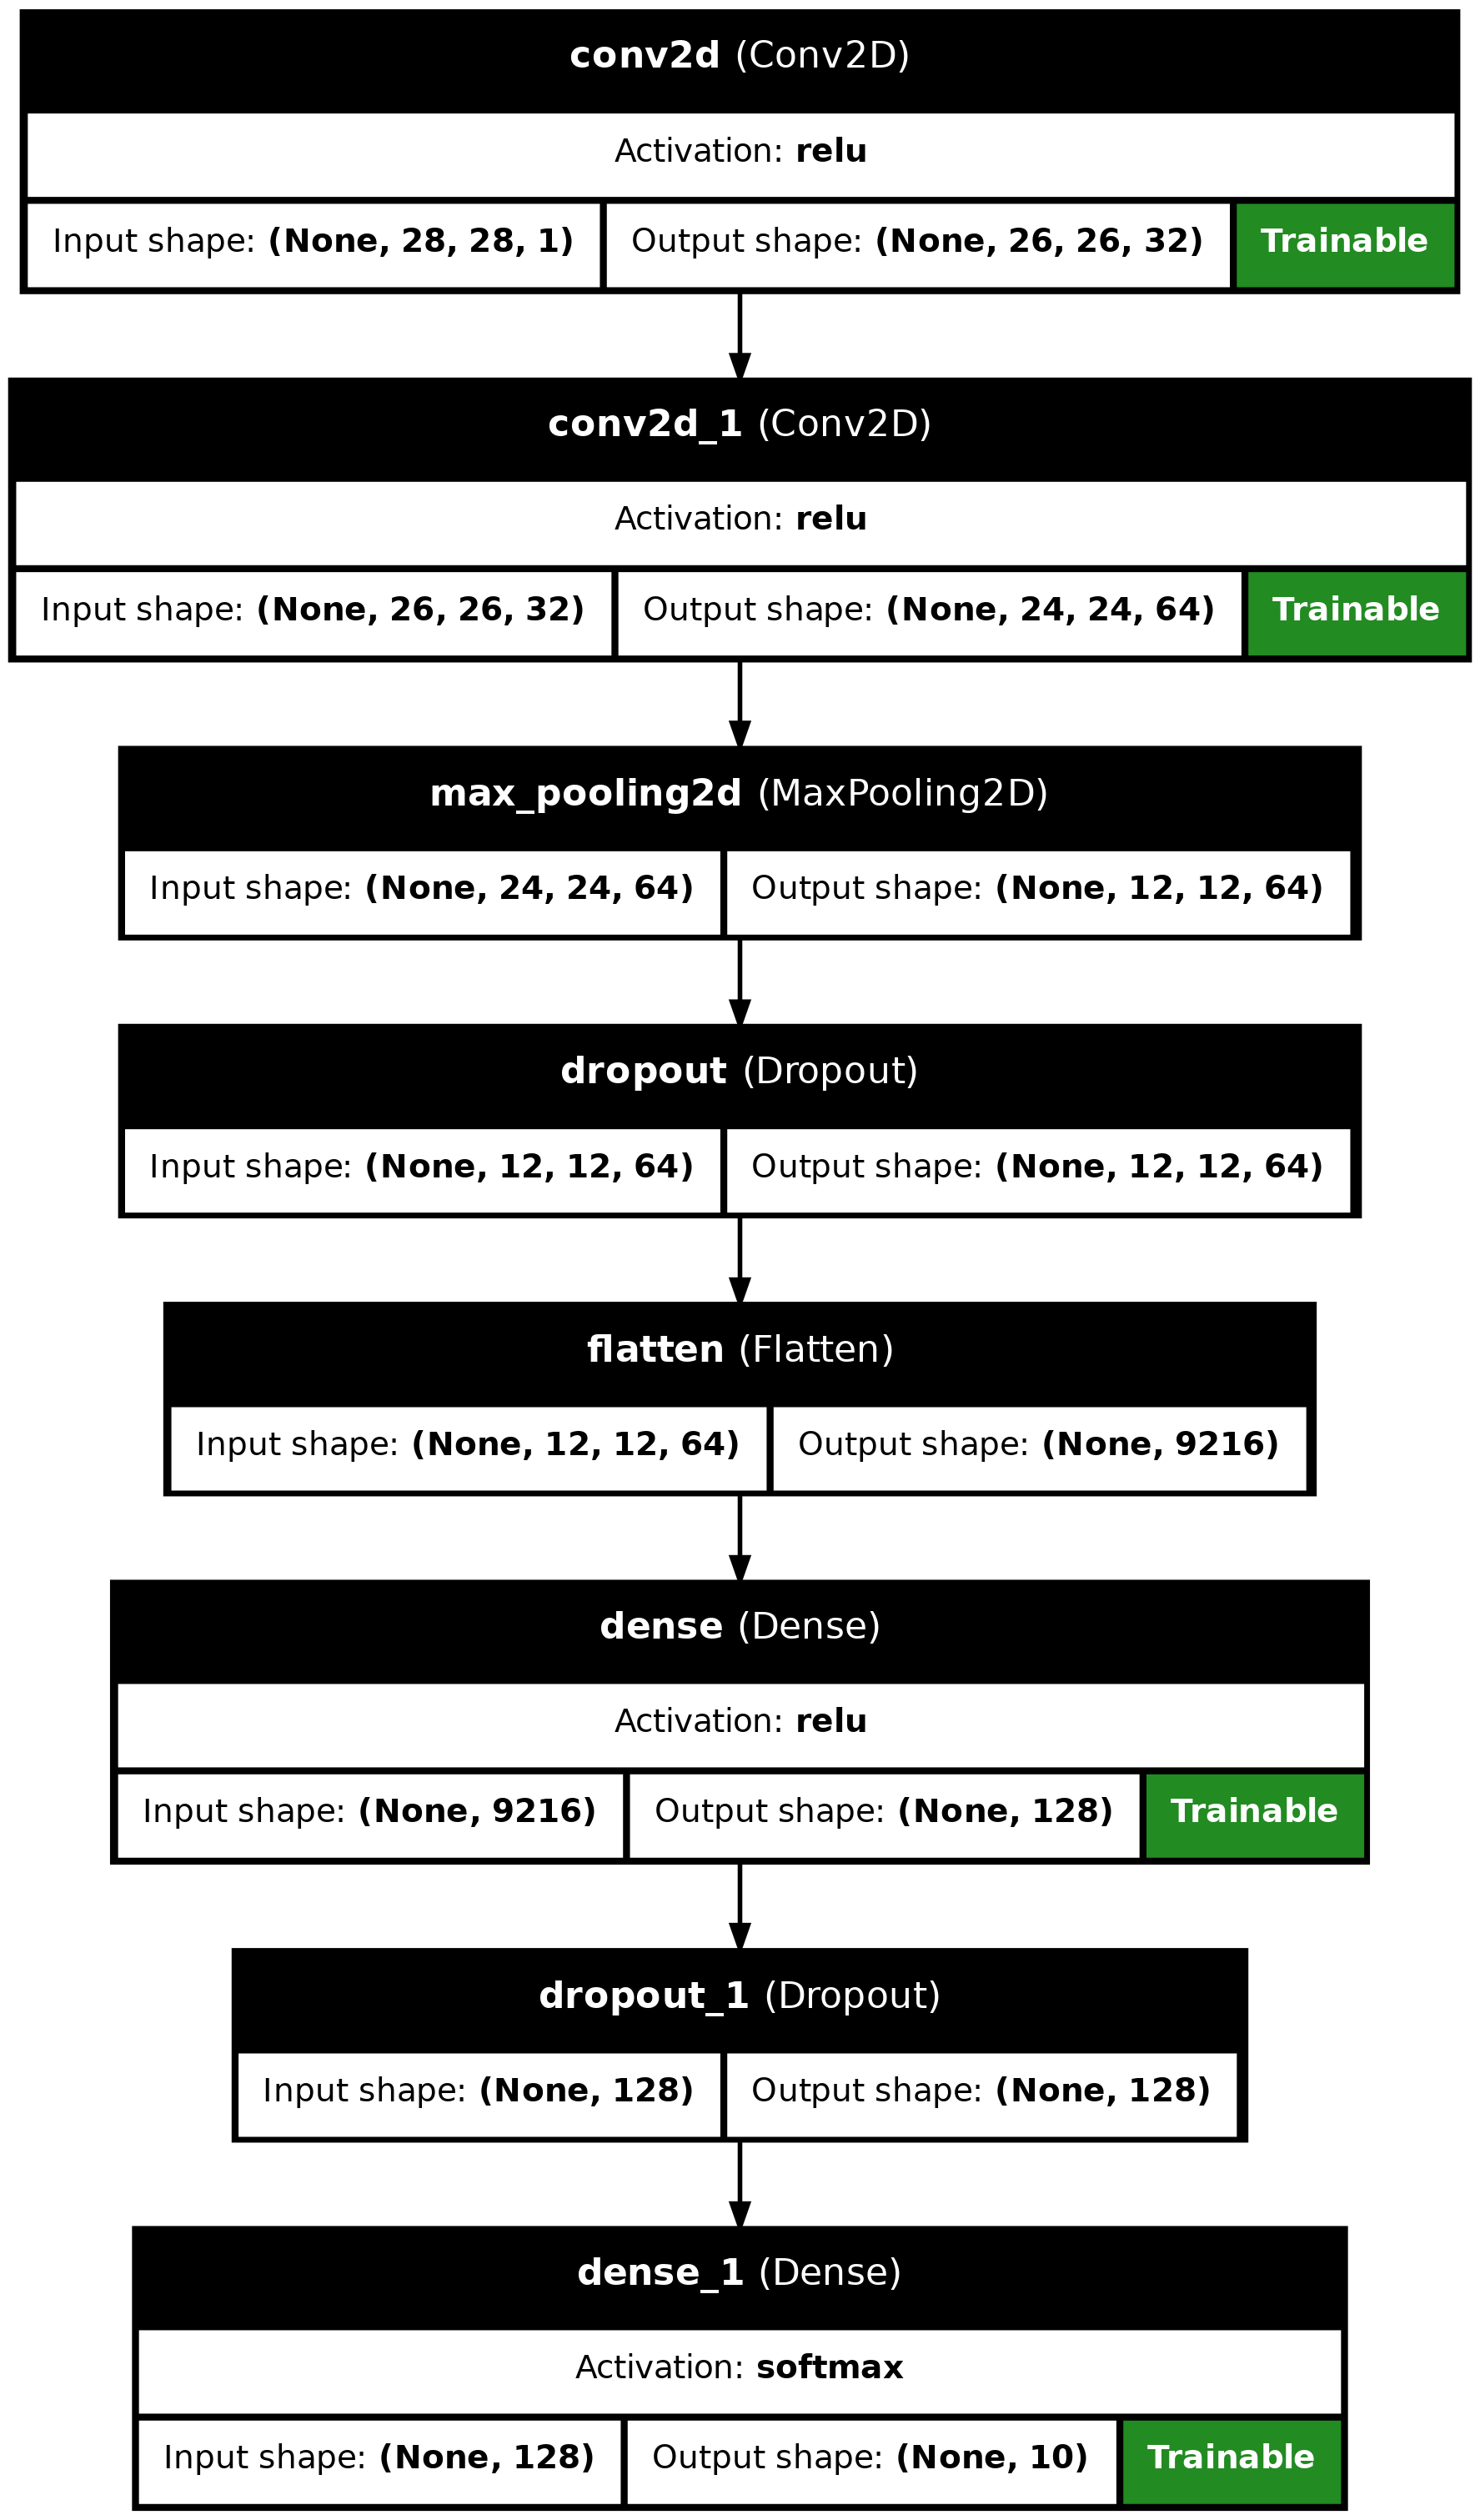
\includegraphics[width=\textwidth]{../images/models/model_cnn_graph.png}
    \caption{Model CNN}
    \label{fig:model_cnn_graph}
  \end{minipage}%
  \hfill
  \begin{minipage}{0.4\textwidth}
    \centering
    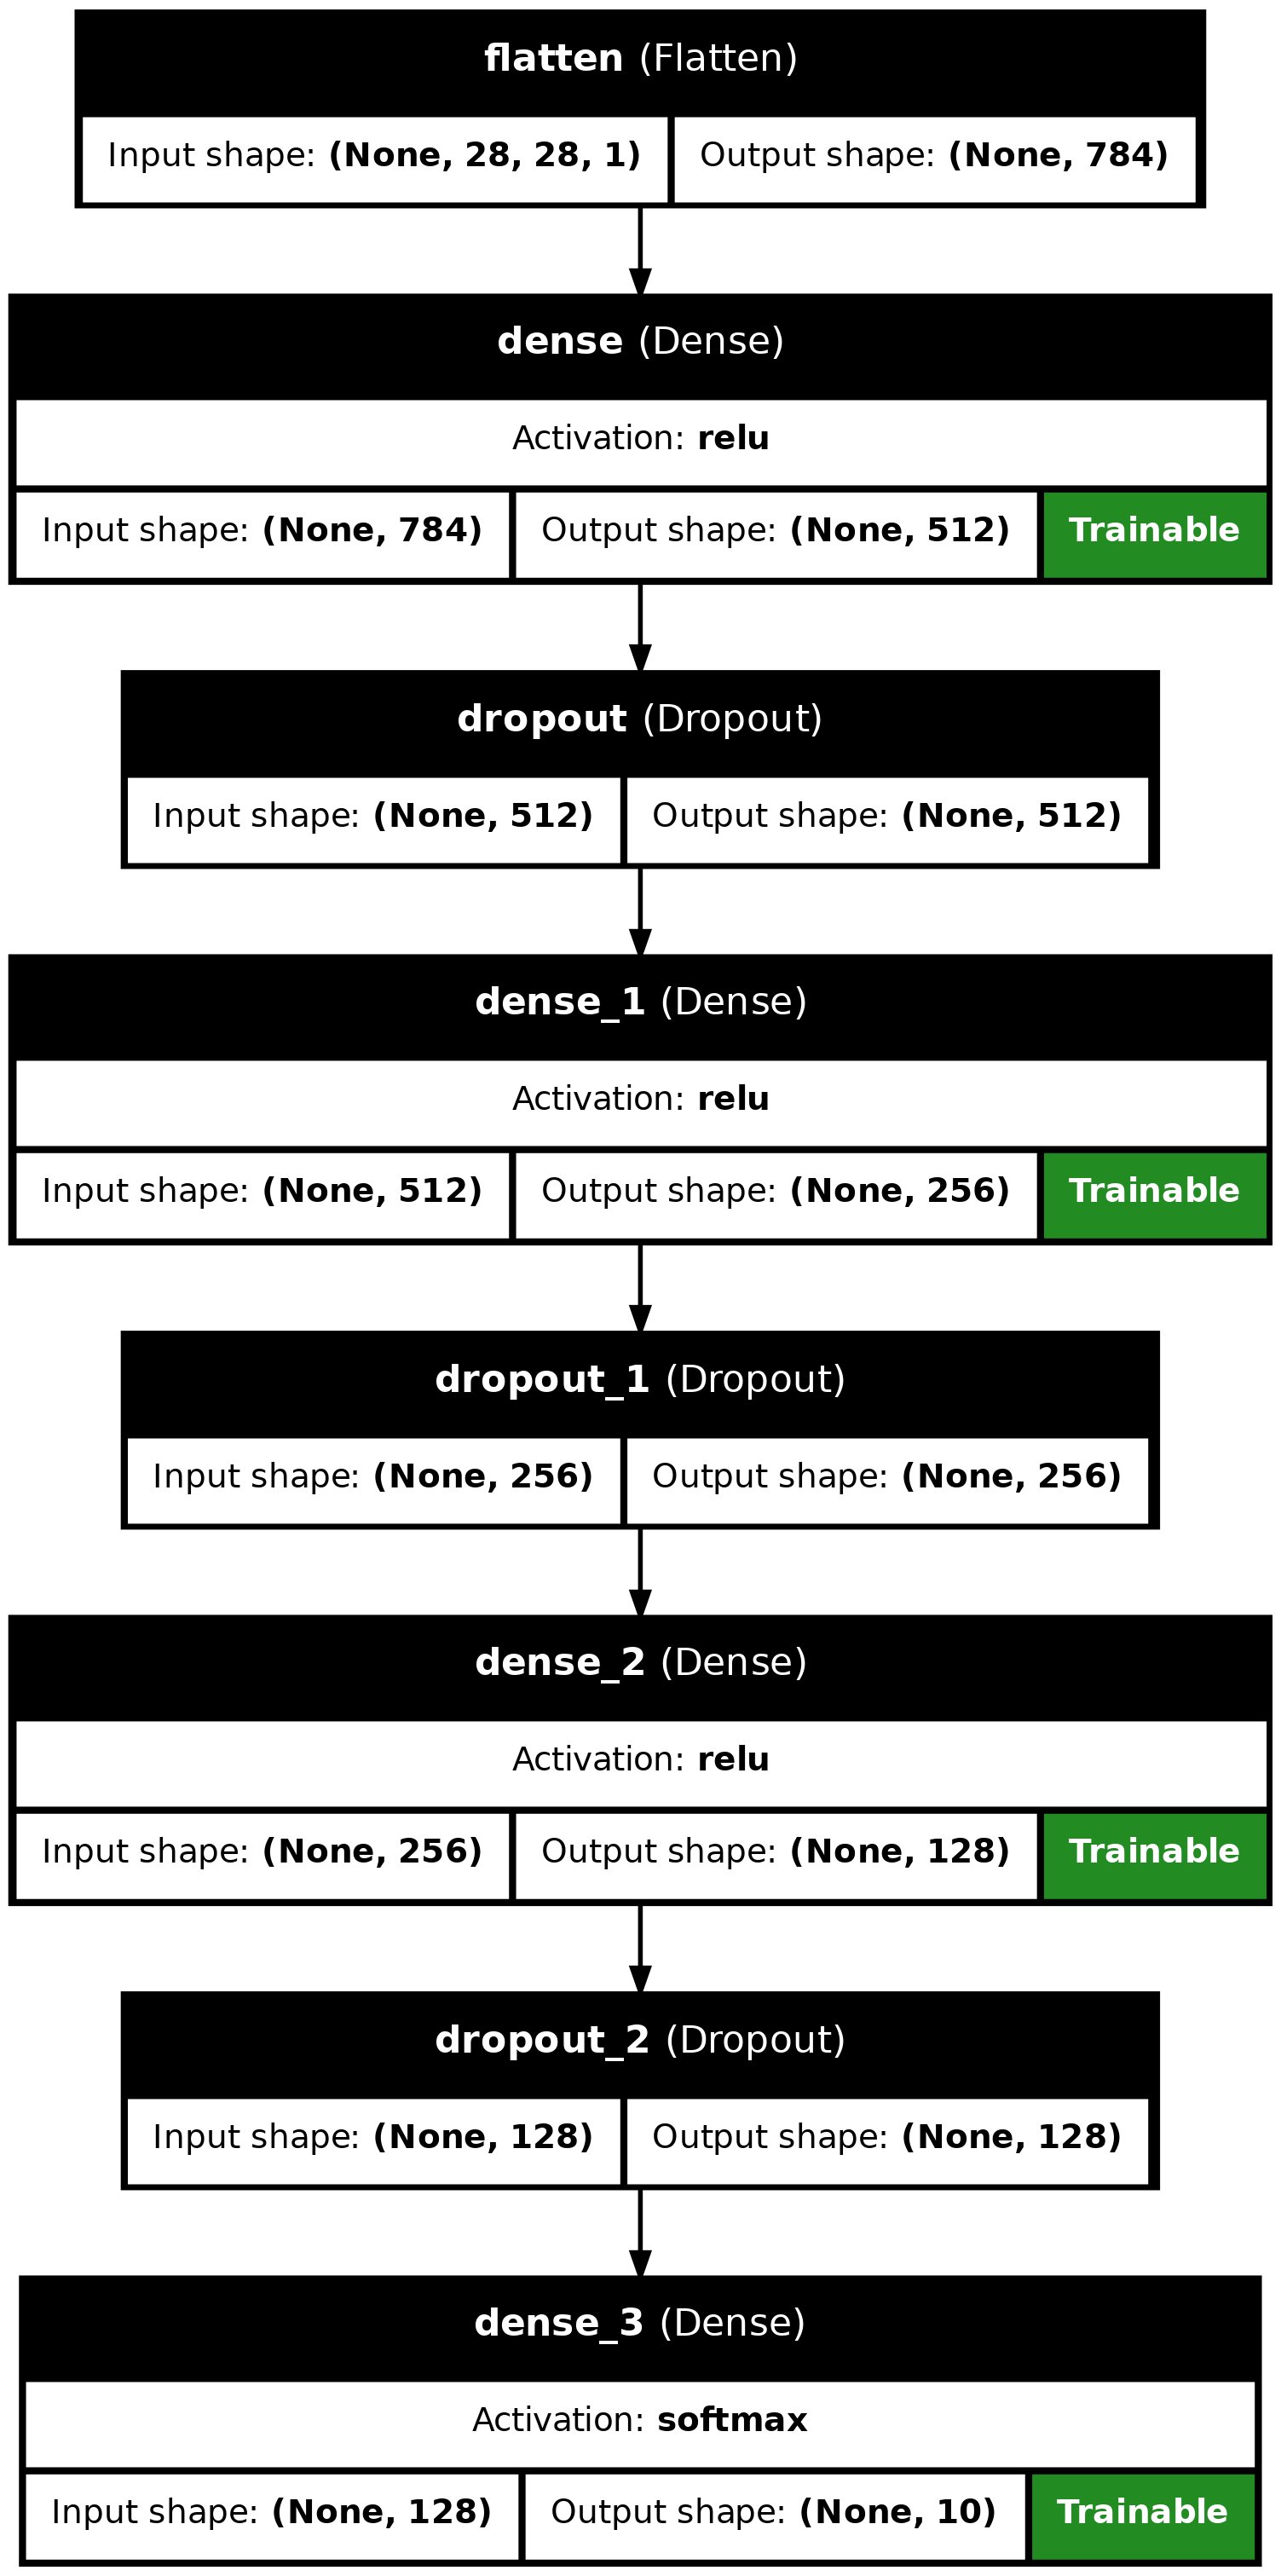
\includegraphics[width=\textwidth]{../images/models/model_fcnn_graph.png}
    \caption{Modelo FCNN}
    \label{fig:model_fcnn_graph}
  \end{minipage}
\end{figure}

Respondendo à Q3, vemos que a principal diferença das implementações realizadas nesse trabalho da CNN e da FCNN são as camadas convolucionais e a camada de polling da CNN. Fora isso, ambas as arquiteturas são similares, já que a CNN possui uma rede fully connected no final dela.

O modelo FCNN contém 1.333.770 parâmetros treináveis, enquanto o modelo CNN tem 1.199.882, mantendo a quantidade de parâmetros similar, como exigido.

Para realizar o treinamento, predição e outras tarefas relacionadas aos modelos anteriores, foi utilizado o tensorflow \cite{tensorflow2015-whitepaper} e keras \cite{chollet2015keras}.

O código utilizadado para a criação da CNN é inspirado no código de uma CNN usada de \textit{benchmark} disponível no repositório do GitHub do Kuzushiji-MNIST (link disponibilizado anteriormente).

Abaixo segue algumas configurações feitas nos modelos, fora as demostradas nas Figuras \ref{fig:model_cnn_graph} e \ref{fig:model_fcnn_graph}:

\begin{enumerate}
  \item \textbf{Early stopping:} Os modelos não possuem um número fixo de épocas para o treinamento, foi estabelecido um número arbitráriamente grande de 10 mil épocas e, quando o valor de loss na validação não diminui em 10 épocas seguidas o treinamento é parado e o melhor modelo escolhido é aquele que possui o menor valor de loss na validação. 
  \item \textbf{Reduce learning rate on plateu:} A taxa de aprendizado dos modelos inicia como 0.001, porém, quando o valor de loss na validação começa a ter poucas variações, essa taxa de aprendizado é reduzida. Isso faz com que os pesos mudem menos ao longo das épocas quando o treinamento está chegando em um mínimo, assim trazendo uma mais precisão. 
  \item \textbf{Função de loss:} A função de loss escolhida foi a \textit{categorical crossentropy}, pois dentro as funções de loss implementadas no keras é a que mais atendia as especificações do projeto.
  \item \textbf{Otimizador:} O otimizador escolhido foi o adadelta
\end{enumerate}


\subsection{Execução do código}

O código utilizado para gerar os resultados apresentados nesse relatório se encontra junto a esse relatório na entrega do trabalho e em um repositório do GitHub \footnote{https://github.com/semcovici/kmnist-classification}. As instruções para a execução se encontram no arquivo README.md na seção ``Instruções".

\section{Resultados}

Na tabela~\ref{table:results_f1}, temos os resultados de \textit{F1-Score} para cada uma das 10 classes no conjunto de teste, bem como o resultado de \textit{F1-Score macro} (média aritimética do \textit{F1-Score} das classes), que nos dá uma visão geral do desempenho do modelo para todas as classes.

\begin{table}[H]\scriptsize\centering
\begin{tabular}{l|rrrrr}
\toprule
classe & CNN & CNN com data augmentation & CNN sem polling & FCNN & FCNN com data augmentation \\
\midrule
0 & 0.9114 & 0.9508 & 0.9168 & 0.9127 & 0.9514 \\
1 & 0.8728 & 0.9042 & 0.8867 & 0.8778 & 0.9107 \\
2 & 0.8483 & 0.8850 & 0.8354 & 0.8409 & 0.8676 \\
3 & 0.9223 & 0.9259 & 0.9202 & 0.9260 & 0.9187 \\
4 & 0.8681 & 0.9034 & 0.8737 & 0.8739 & 0.9112 \\
5 & 0.9013 & 0.9263 & 0.8976 & 0.9074 & 0.9232 \\
6 & 0.8765 & 0.9272 & 0.8906 & 0.8890 & 0.8996 \\
7 & 0.9038 & 0.9444 & 0.9025 & 0.9008 & 0.9471 \\
8 & 0.8694 & 0.9170 & 0.8773 & 0.8763 & 0.9211 \\
9 & 0.9002 & 0.9388 & 0.9016 & 0.8994 & 0.9409 \\
\midrule
macro avg & 0.8874 & 0.9223 & 0.8902 & 0.8904 & 0.9192 \\
\bottomrule
\end{tabular}

    
\caption{Resultados de \textit{F1-Score} no conjunto de teste (arredondados em 4 casas decimais)}
\label{table:results_f1}
\end{table}

É possível observar que, em todos os modelos, o desempenho em cada classe é bastante consistente, não havendo classes que apresentam uma grande vantagem em detrimento de outras e, também, não há classes em grande desvantagem.

Considerando o \textit{F1-Score macro}, vemos que os diferentes experimentos não causaram grandes diferenças nos resultados, sendo o pior resultado da CNN com 88,74\% de \textit{F1-Score macro} e o melhor da CNN com \textit{data augmentation}, com 92,23\%.

A remoção da camada de pooling traz ganhos aparentemente não significativos ao desempenho do modelo no conjunto de teste, tendo em vista que há uma diferença de aproximadamente 0,26\% nos resultados. Já a adição de \textit{data augmentation} se mostra eficiente na melhoria do desempenho nos dois algoritmos testados, FCNN e CNN.

Por outro lado, ao observar a curva de aprendizado da CNN (Figura \ref{fig:cnn_loss_progress}) e da FCNN (Figura \ref{fig:fcnn_loss_progress}), vemos que a CNN converge por volta de 600 épocas, enquanto a FCNN precisa de quase o dobro de épocas para convergir.

\begin{figure}[H]
\centering
\begin{minipage}{0.5\textwidth}
  \centering
  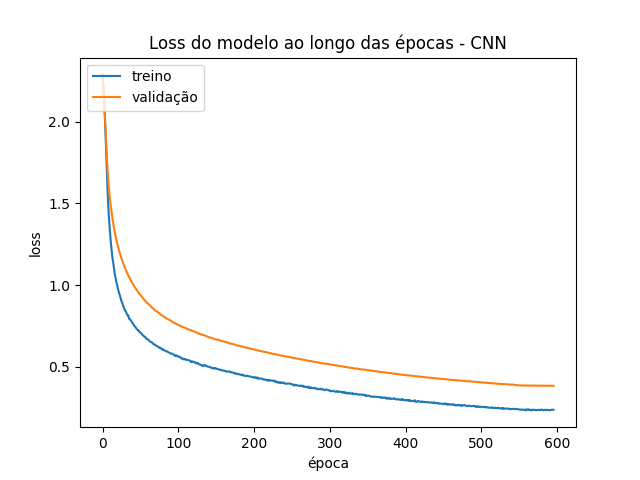
\includegraphics[width=\textwidth]{../images/results_plt/cnn_loss_progress.png}
  \caption{Curva de aprendizado CNN}
  \label{fig:cnn_loss_progress}
\end{minipage}%
\hfill
\begin{minipage}{0.5\textwidth}
  \centering
  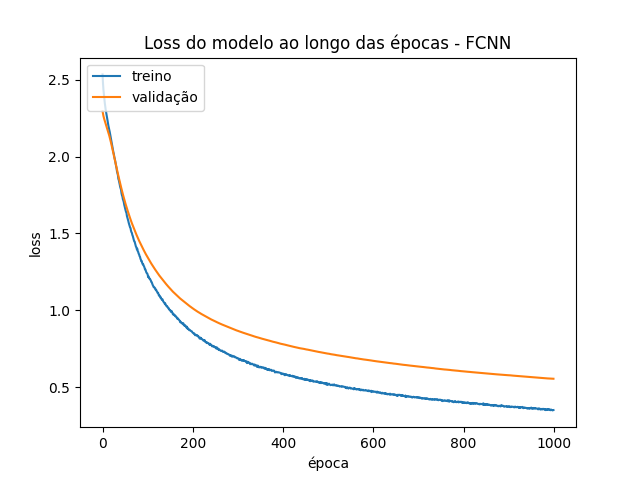
\includegraphics[width=\textwidth]{../images/results_plt/fcnn_loss_progress.png}
  \caption{Curva de aprendizado FCNN}
\label{fig:fcnn_loss_progress}
\end{minipage}
\end{figure}

A remoção da camada de pooling da CNN faz o modelo convergir mais rápido, porém vemos um \textit{overfitting} do modelo no treino, com um \textit{loss} menor que 0,25 no conjunto de treino ao final do treinamento, que é inferior ao \textit{loss} final do conjunto de treino na CNN tradicional, conforme mostrado na Figura \ref{fig:cnn_sem_polling_loss_progress}. Assim, responde-se à Q5.

\begin{figure}[ht]
  \centering
  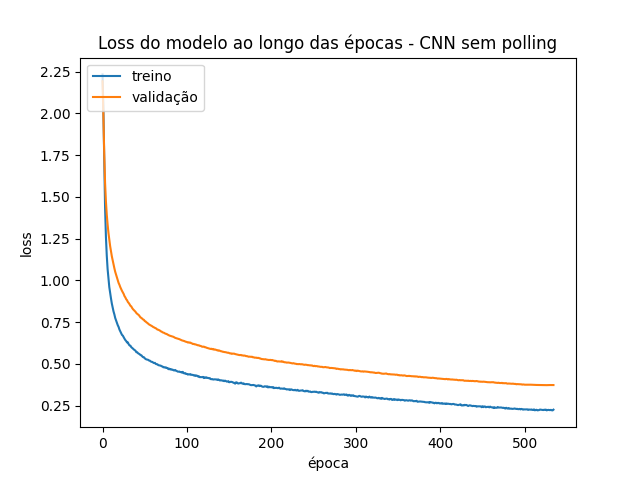
\includegraphics[width=.5\textwidth]{../images/results_plt/cnn_sem_polling_loss_progress.png}
  \caption{Curva de aprendizado CNN sem polling}
  \label{fig:cnn_sem_polling_loss_progress}
\end{figure}

A adição de \textit{data augmentation} na CNN traz uma redução drástica do \textit{overfitting} do modelo no treinamento, com o \textit{loss} ao longo das épocas no treino e validação bem próximos, conforme mostrado na Figura \ref{fig:cnn_com_data_augmentation_loss_progress}. Já na FCNN, a adição de \textit{data augmentation} também traz uma redução no \textit{overfitting}, porém não tanto quanto na CNN, conforme mostrado na Figura \ref{fig:fcnn_com_data_augmentation_loss_progress}. Além disso, a adição de \textit{data augmentation} demonstra uma redução no número de épocas para convergir. Em contraponto a isso, a adição de mais dados torna o treinamento computacionalmente mais custoso, de forma que a redução de épocas não diminui o tempo de treinamento.

\begin{figure}[H]
  \centering
  \begin{minipage}{0.5\textwidth}
    \centering
    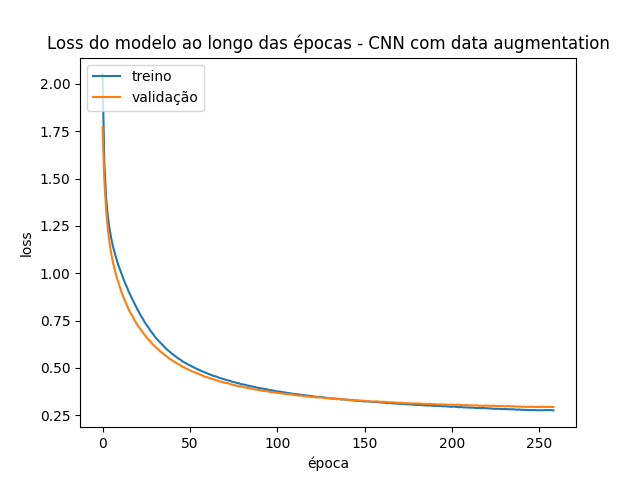
\includegraphics[width=\textwidth]{../images/results_plt/cnn_com_data_augmentation_loss_progress.png}
    \caption{Curva de aprendizado CNN com \textit{data augmentation}}
    \label{fig:cnn_com_data_augmentation_loss_progress}
  \end{minipage}%
  \hfill
  \begin{minipage}{0.5\textwidth}
    \centering
    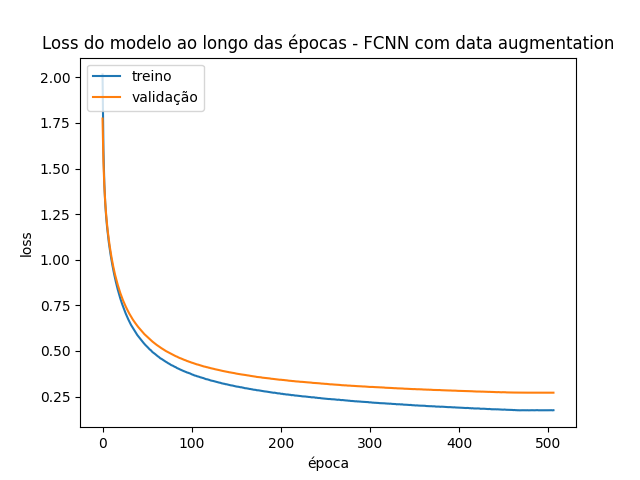
\includegraphics[width=\textwidth]{../images/results_plt/fcnn_com_data_augmentation_loss_progress.png}
    \caption{Curva de aprendizado FCNN com \textit{data augmentation}}
    \label{fig:fcnn_com_data_augmentation_loss_progress}
  \end{minipage}
\end{figure}


Para responder à Q6 e à Q7, nas Figuras \ref{fig:model_cnn_layer_0_kernel_plot} e \ref{fig:model_cnn_layer_1_kernel_plot}, temos os filtros formados após o treinamento do modelo CNN nas camadas convolucionais. Não há um padrão interpretável nesses filtros que mostre algum aspecto que o modelo aprendeu nas imagens. Isso não significa que o modelo não aprendeu nada, apenas que a análise dos filtros gerados não resulta em um melhor entendimento do funcionamento do modelo.

\begin{figure}[H]
  \centering
  \begin{minipage}{0.5\textwidth}
    \centering
    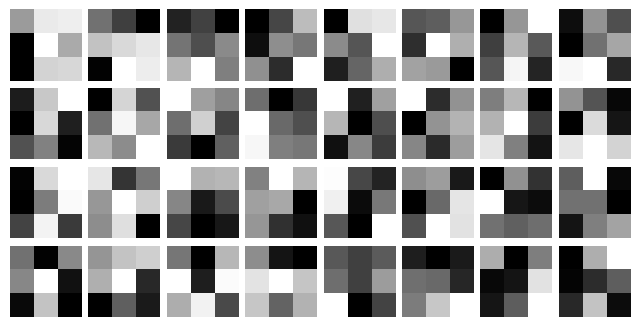
\includegraphics[width=.5\textwidth]{../images/kernels_plt/model_cnn_layer_0_kernel_plot.png}
    \caption{Filtros da primeira camada convolucional do modelo de CNN}
    \label{fig:model_cnn_layer_0_kernel_plot}
  \end{minipage}%
  \hfill
  \begin{minipage}{0.5\textwidth}
    \centering
    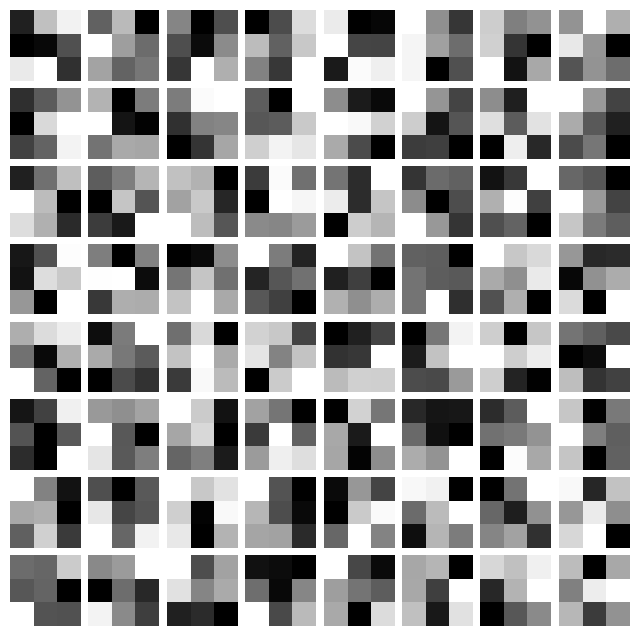
\includegraphics[width=.5\textwidth]{../images/kernels_plt/model_cnn_layer_1_kernel_plot.png}
    \caption{Filtros da segunda camada convolucional do modelo de CNN}
    \label{fig:model_cnn_layer_1_kernel_plot}
  \end{minipage}
  \end{figure}

  Esse padrão de ``filtros não interpretáveis" se repete  na versão sem camada de polling e na versão com \textit{data augmentation}.

  Respondendo às Q4 e Q8, é importante entender as diferenças entre os pesos de uma rede fully connected e os filtros de uma CNN no processo de extração de características. Os filtros em uma CNN aplicam convoluções diretamente sobre as imagens, extraindo padrões locais, como bordas, texturas e formas, de maneira eficiente e preservando a estrutura espacial da imagem. Embora os filtros não sejam sempre interpretáveis visualmente, como mostrado anteriormente, eles são visualizáveis e oferecem uma compreensão parcial do que o modelo está aprendendo. Por outro lado, os pesos em uma rede fully connected não possuem essa representatividade visual direta, pois cada neurônio está conectado a todos os pixels, e as imagens geralmente passam por uma etapa de \textit{flatten}, que converte a imagem em um vetor unidimensional. Esse processo faz com que as informações espaciais da imagem original sejam perdidas, tornando mais difícil interpretar os padrões aprendidos pela rede.

  As CNNs, ao se concentrarem em regiões locais da imagem através das convoluções, capturam melhor as informações espaciais em comparação às fully connected, que tratam todos os pixels de forma global e independente. Além disso, as CNNs reduzem significativamente o número de parâmetros treináveis, tornando o modelo mais eficiente e menos propenso ao \textit{overfitting}. Assim, enquanto as redes fully connected oferecem maior flexibilidade, as CNNs são mais eficazes na tarefa de extração de características visuais, o que explica seu melhor desempenho em tarefas relacionadas a imagens. Dessa forma, a diferença fundamental entre os pesos de uma fully connected e os filtros de uma CNN está na capacidade de representação e extração de padrões relevantes para a classificação de imagens.

\section{Conclusão e limitações}

Neste trabalho, foram explorados alguns experimentos para comparar a capacidade de aprendizado na tarefa de classificação entre redes neurais \textit{fully connected} (FCNN) e redes neurais convolucionais (CNN). Os resultados obtidos no conjunto de treino de ambas as arquiteturas são bastante similares, embora a CNN tenha um desempenho levemente inferior. Entretanto, a FCNN demora mais para convergir, necessitando de mais de 1,1 mil épocas para estabilizar, enquanto a CNN converge em aproximadamente 600 épocas, respondendo assim à Q1.

Além disso, foi testada a técnica de \textit{data augmentation}, que trouxe uma melhoria nos resultados de ambas as arquiteturas no conjunto de teste. No entanto, a CNN com \textit{data augmentation} obteve um desempenho levemente superior à FCNN.

Por fim, testou-se a remoção da camada de pooling da CNN, que não resultou em grandes ganhos e causou um aumento no \textit{overfitting} durante o treino.

Dessa forma, neste trabalho foram exploradas todas as questões solicitadas como "Exploração mínima esperada" e "Exploração adicional". Contudo, não foi possível investigar, dentro do prazo estipulado, as mudanças nos hiperparâmetros mencionadas ao final da seção "Exploração adicional". A única questão abordada dessa seção foi a aplicação de \textit{data augmentation}.

\bibliographystyle{sbc}
\bibliography{sbc-template}

\end{document}
